\section{Circuitos de corriente directa}
  \subsection{Fuerza electromotriz}
    \PN Dado que en un circuito particular la diferencia de potencial en las terminales de la batería es constante, la
    corriente en el circuito es constante en magnitud y dirección y recibe el nombre de corriente directa. A la batería se
    le conoce como fuente de fuerza electromotriz, o más comúnmente, \textit{fuente de fem}. (Lo que se conoce como
    \textbf{fuerza electromotriz} es un desafortunado equívoco histórico, pues describe no una fuerza, sino una diferencia
    de potencial en volts.) La fem $\varepsilon$ de una batería es el voltaje máximo posible que ésta puede suministrar
    entre sus terminales.

    \begin{figure}[H]
    \centering
      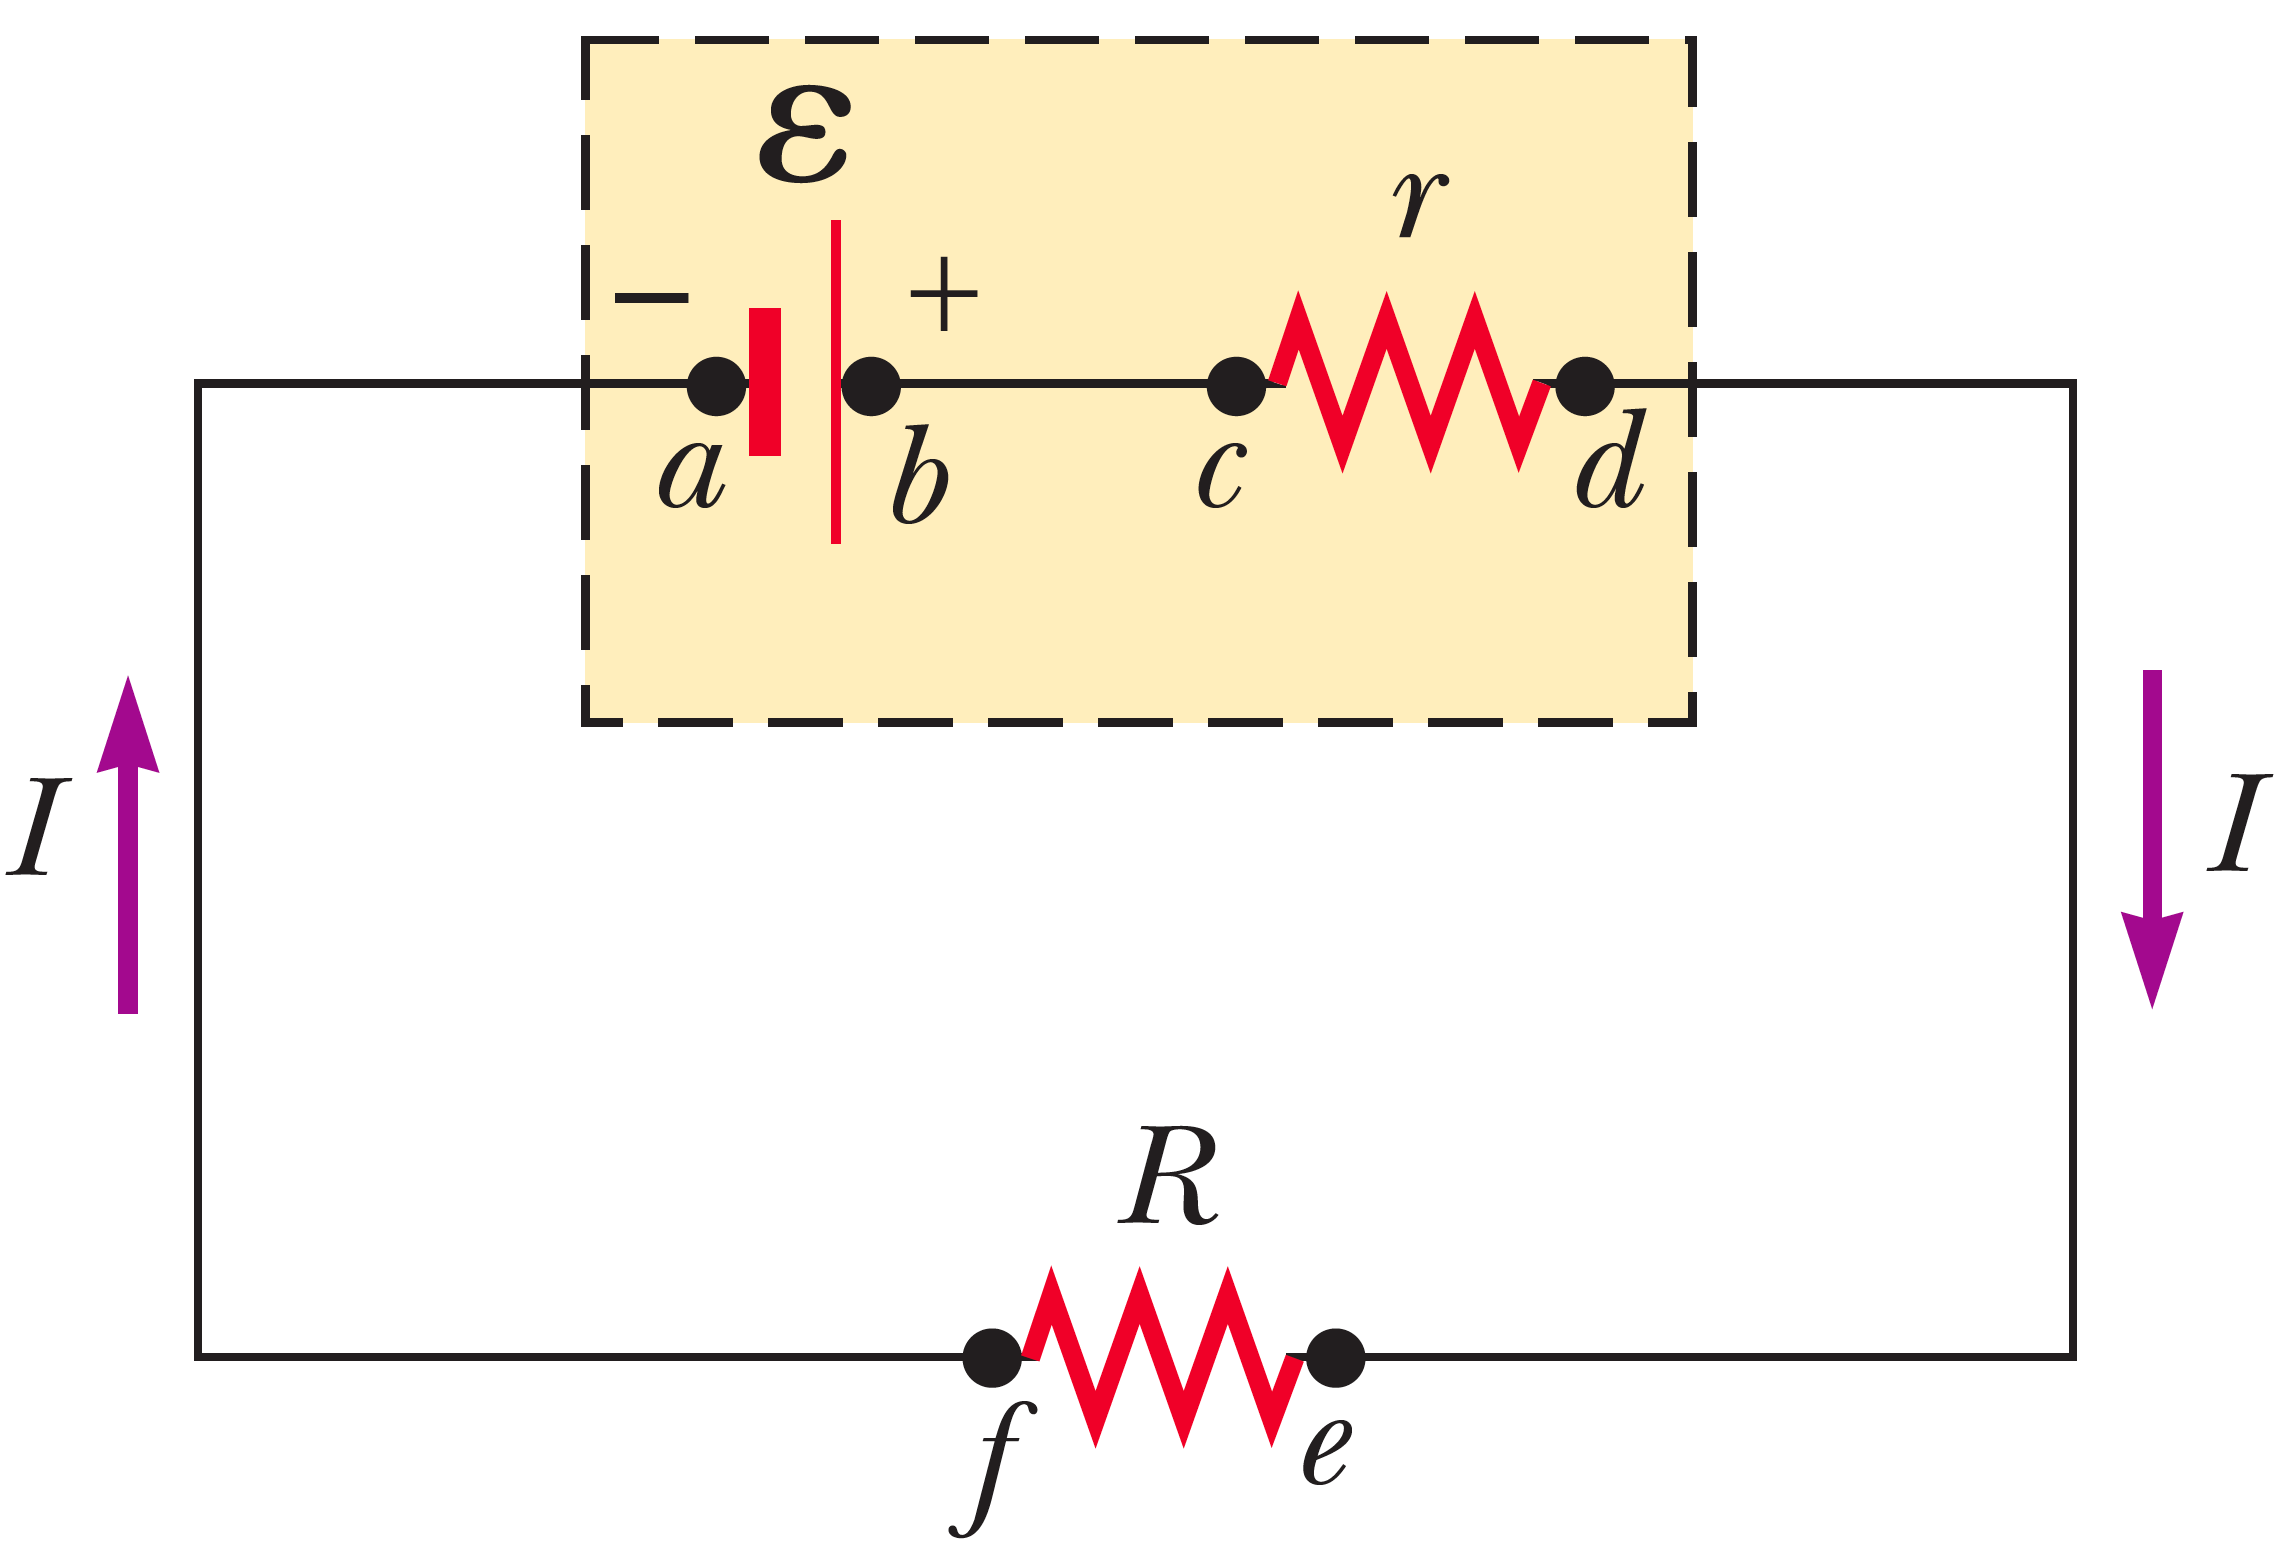
\includegraphics[width=0.35\textwidth]{4/figure_10}
      \caption{Diagrama de un circuito de una fuente de fem $\varepsilon$ (en este caso, una batería), de resistencia
      interna $r$, conectada a un resistor externo, de resistencia $R$.}
    \end{figure}

    \PN La terminal positiva de la batería se encuentra a un potencial más alto que la negativa. Puesto que una batería
    está hecha de materia, existe una resistencia al flujo de las cargas dentro de la misma. Esta resistencia recibe el
    nombre de \textbf{resistencia interna} $r$. En el caso de una batería ideal con una resistencia interna igual a cero,
    la diferencia de potencial a través de la batería (conocida como voltaje entre las terminales) es igual a su fem. El
    el voltaje entre las terminales de la batería $\Delta V = V_{d} - V_{a}$ es:
    \begin{equation*}
      \Delta V = \varepsilon - I r
    \end{equation*}

    \PN Notar que $\varepsilon$ es equivalente al \textbf{voltaje en circuito abierto}, es decir, el voltaje entre las
    terminales cuando la corriente es igual a cero. La diferencia de potencial real entre las terminales de la batería
    depende de la corriente en la misma.

    \VS
    \PN El voltaje entre las terminales $\Delta V$ debe ser igual a la diferencia de potencial de un extremo a otro de la
    resistencia externa $R$, conocida como \textbf{resistencia de carga}. El resistor representa una carga en la batería
    porque ésta debe suministrar energía para que el aparato que contiene la resistencia funcione. La diferencia de
    potencial de un extremo a otro de la resistencia de carga es $\Delta V = IR$.
    \begin{equation*}
      \varepsilon = IR + Ir
    \end{equation*}

    \PN Al resolver en función de la corriente
    \begin{equation*}
      I = \frac{\varepsilon}{R + r}
    \end{equation*}

    \PN Esta ecuación muestra que la corriente en este circuito simple depende tanto de la resistencia de carga $R$
    externa a la batería como de la resistencia interna $r$. Si $R$ es mucho mayor que $r$, como es el caso de muchos
    circuitos útiles en la vida cotidiana, ignore $r$, es decir:
    \begin{equation*}
      \varepsilon = IR
    \end{equation*}

  \subsection{Resistores en serie y en paralelo}
    \subsubsection{Resistores en serie}

      \begin{figure}[H]
      \centering
        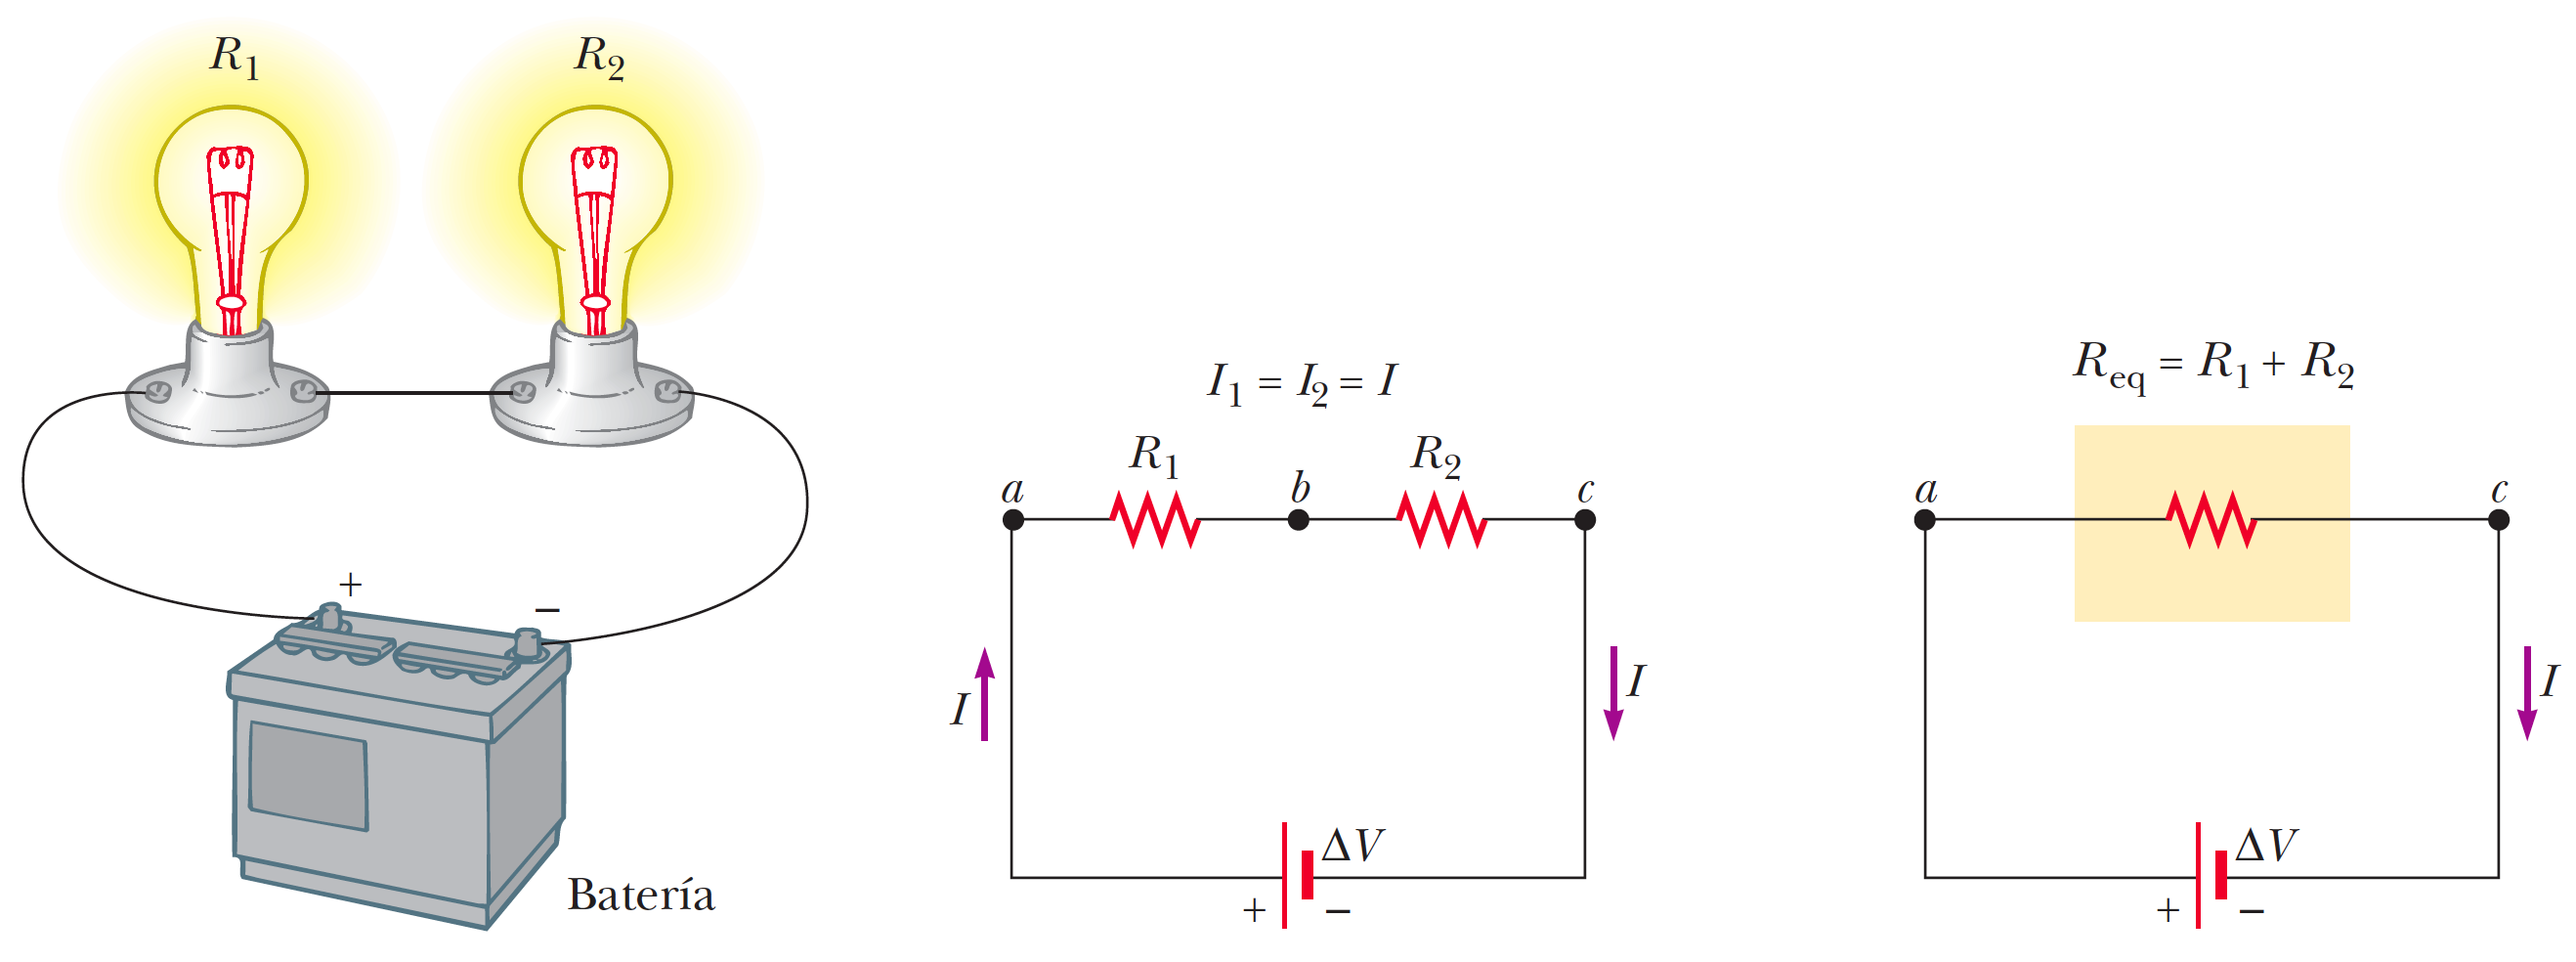
\includegraphics[width=0.7\textwidth]{4/figure_11}
        \caption{Diagrama de un circuito de una fuente de fem $\varepsilon$ (en este caso, una batería), de resistencia
        interna $r$, conectada a un resistor externo, de resistencia $R$.}
      \end{figure}

      \PN Cuando dos o más resistores están interconectados como los de la figura anterior, se dice que están en una
      \textbf{combinación en serie}. En una conexión en serie, si una cantidad de carga $Q$ sale de un resistor $R_{1}$,
      deberá también entrar en el segundo resistor $R_{2}$. Por lo tanto, en un intervalo determinado de tiempo, la
      misma cantidad de carga pasa a través de ambos resistores.
      \begin{equation*}
        I = I_{1} = I_{2}
      \end{equation*}

      \PN donde $I$ es la corriente de la batería, $I_{1}$ es la corriente en el resistor $R_{1}$ e $I_{2}$ es la
      corriente en el resistor $R_{2}$.

      \VS
      \PN La diferencia de potencial que se aplica a una combinación en serie de resistores se dividirá entre éstos. En
      la figura, ya que la caída de voltaje de $a$ a $b$ es igual a $I_{1}R_{1}$ y la caída de voltaje de $b$ a $c$ es
      \begin{equation*}
        \Delta V = I_{1}R_{1} + I_{2}R_{2}
      \end{equation*}

      \PN La diferencia de potencial entre las terminales de la batería también está aplicada a la resistencia
      equivalente $R_{eq}$:
      \begin{equation*}
        \Delta V = I R_{eq}
      \end{equation*}

      \PN donde la resistencia equivalente tiene el mismo efecto en el circuito que en la combinación en serie porque
      resulta de la misma corriente $I$ en la batería. Al combinar estas ecuaciones para $\Delta V$ se sustituyen los
      dos resistores en serie por una sola resistencia equivalente, cuyo valor es la \textit{suma} de las resistencias
      equivalentes:
      \begin{equation*}
        \Delta V = I R_{eq} = I_{1}R_{1} + I_{2}R_{2} \rightarrow R_{eq} = R_{1} + R_{2}
      \end{equation*}

      \PN La resistencia equivalente de tres o más resistores conectados en serie es
      \begin{equation*}
        R_{eq} = R_{1} + R_{2} + R_{3} + \dotsc
      \end{equation*}

      \PN Esta correspondencia indica que \textbf{la resistencia equivalente de una combinación en serie de resistores
      es la suma numérica de las resistencias individuales y siempre es mayor que cualquier resistencia individual}.

    \subsubsection{Resistores en paralelo}

      \begin{figure}[H]
      \centering
        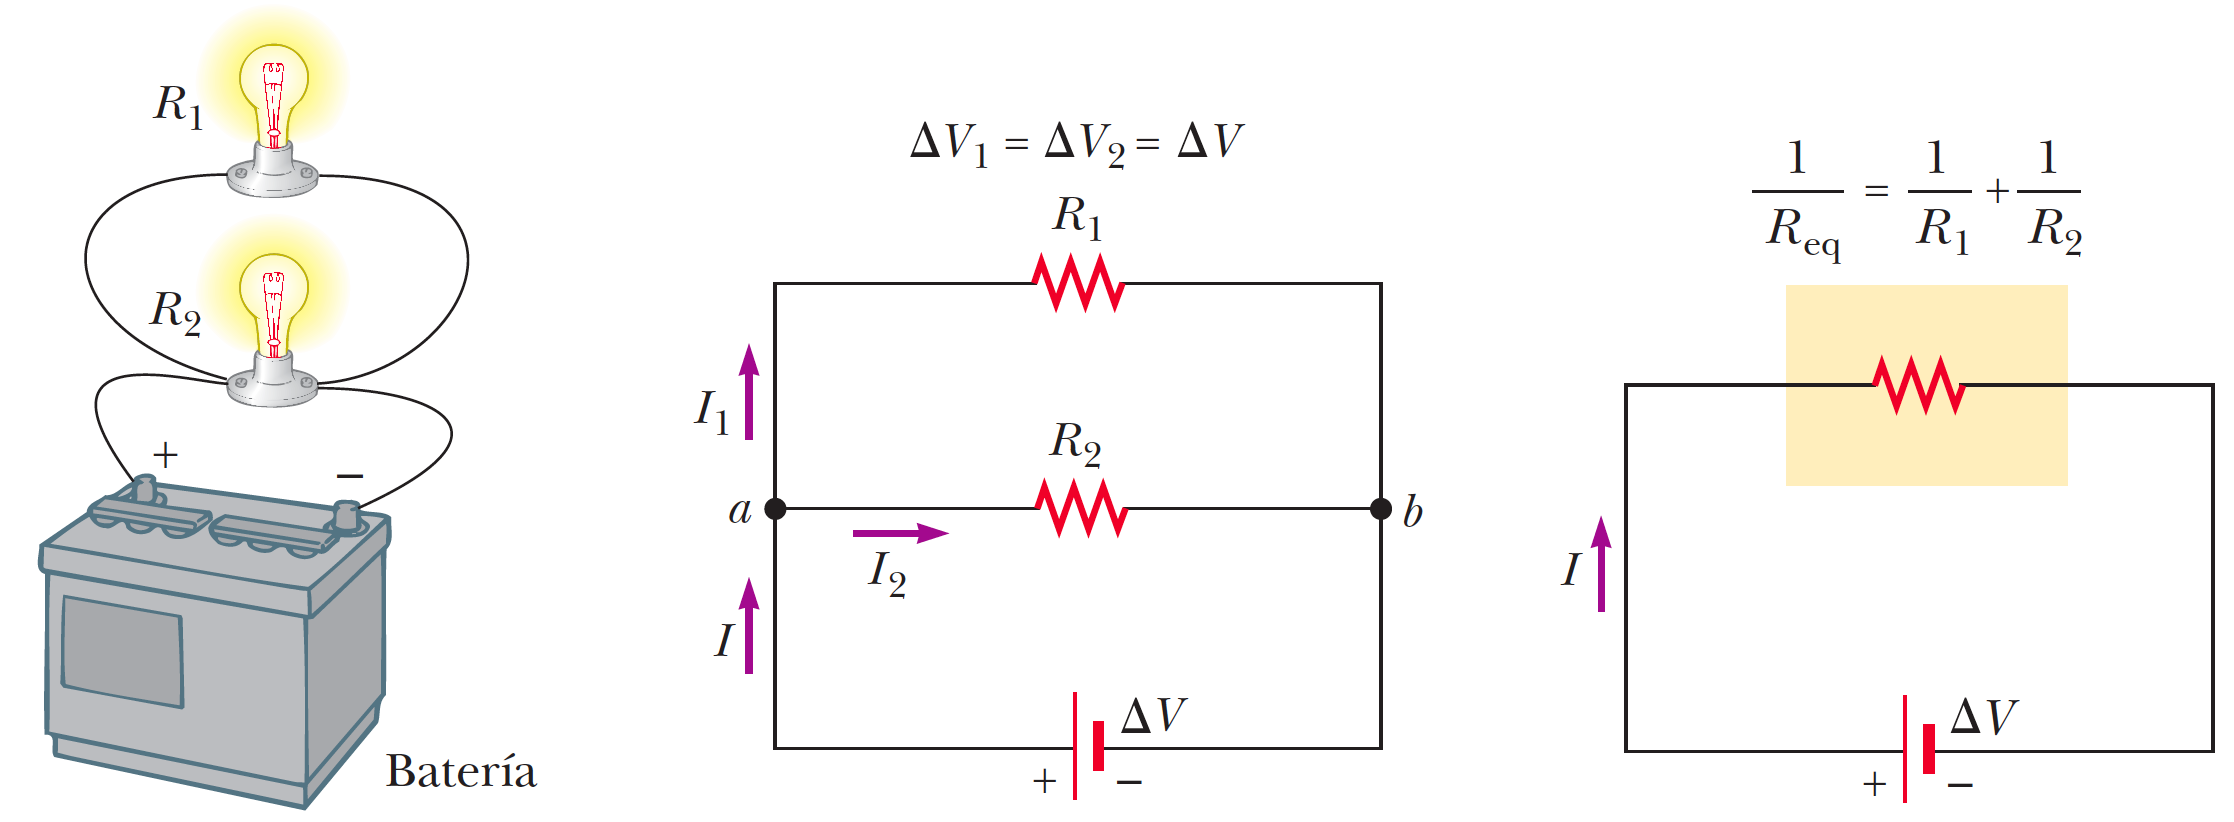
\includegraphics[width=0.7\textwidth]{4/figure_12}
        \caption{Diagrama de un circuito de una fuente de fem $\varepsilon$ (en este caso, una batería), de resistencia
        interna $r$, conectada a un resistor externo, de resistencia $R$.}
      \end{figure}

      \PN En una \textbf{combinación en paralelo}, las diferencias de potencial a través de los resistores son las
      mismas:
      \begin{equation*}
        \Delta V = \Delta V_{1} = \Delta V_{2}
      \end{equation*}

      \PN donde $\Delta V$es el voltaje entre las terminales de la batería.

      \VS
      \PN Cuando las cargas llegan al punto $a$ en la figura b), se dividen en dos; una parte pasa a través de $R_{1}$ y
      el resto a través de $R_{2}$. Una unión es cualquier punto en un circuito donde una corriente puede dividirse.
      Esta división resulta en menos corriente en cada resistor de la que sale de la batería. Debido a que la carga
      eléctrica se conserva, la corriente $I$ que entra al punto a debe ser igual a la corriente total que sale del
      mismo:
      \begin{equation*}
        I = I_{1} + I_{2}
      \end{equation*}

      \PN donde $I_{1}$ es la corriente en $R_{1}$ e $I_{2}$ es la corriente en $R_{2}$.

      \VS
      \PN La corriente en la resistencia equivalente $R_{eq}$ es
      \begin{equation*}
        I = \frac{\Delta V}{R_{eq}}
      \end{equation*}

      \PN donde la resistencia equivalente tiene el mismo efecto en el circuito que las dos resistencias en paralelo,
      por lo que la resistencia equivalente de dos resistores en paralelo se conoce por
      \begin{equation*}
        I = \frac{\Delta V}{R_{eq}} = \frac{\Delta V_{1}}{R_{1}} + \frac{\Delta V_{2}}{R_{2}} \rightarrow
        \frac{1}{R_{eq}} = \frac{1}{R_{1}} + \frac{1}{R_{2}}
      \end{equation*}

      \PN Una extensión de esta explicación a tres o más resistores en paralelo da:
      \begin{equation*}
        \frac{1}{R_{eq}} = \frac{1}{R_{1}} + \frac{1}{R_{2}} + \frac{1}{R_{3}} + \dotsc
      \end{equation*}

      \PN De esta expresión se ve que \textbf{el inverso de la resistencia equivalente de dos o más resistores
      conectados en una combinación en paralelo es igual a la suma de los inversos de las resistencias individuales.
      Además, la resistencia equivalente siempre es menor que la resistencia más pequeña en el grupo}.

    \subsection{Leyes de Kirchhoff}
      \PN Es posible simplificar y explicar combinaciones de resistores aplicando la expresión $\Delta V = IR$ y las
      reglas para las combinaciones en serie y en paralelo de los resistores. Muy a menudo, sin embargo, no es posible
      simplificar un circuito en una sola espira. El procedimiento para explicar circuitos más complejos se hace
      posible si se utilizan dos principios conocidos como leyes de Kirchhoff:

      \begin{itemize}
        \item \textbf{Ley de la unión:} En cualquier unión, la suma de las corrientes debe ser igual a cero:
        \begin{equation*}
          \sum_{union} I = 0
        \end{equation*}

        \item \textbf{Ley de la espira:} La suma de las diferencias de potencial a través de todos los elementos
        alrededor de cualquier espira de un circuito cerrado debe ser igual a cero:
        \begin{equation*}
          \sum_{espira} \ \Delta V = 0
        \end{equation*}
      \end{itemize}

      \PN La primera ley de Kirchhoff es un enunciado de la conservación de la carga eléctrica. La segunda ley de
      Kirchhoff es una consecuencia de la ley de conservación de energía.

      \VS
      \PN Las siguientes son reglas para determinar las diferencias de potencial a través de un resistor y de una
      batería, utilizando la segunda ley y bajo la supocición de que la batería no tiene resistencia interna. Cada
      elemento del circuito se recorre de $a$ hasta $b$, de izquierda a derecha.
      \begin{multicols}{2}
        \begin{itemize}
          \item las cargas se mueven del extremo de potencial alto de un resistor hacia el extremo de potencial bajo; si
          un resistor se atraviesa en la dirección de la corriente, la diferencia de potencial $\Delta V$ a través del
          resistor es $-IR$ (figura a)).
          \item si un resistor se recorre en la dirección opuesta a la corriente, la diferencia de potencial $\Delta V$ a
          través del resistor es $+IRR$ (figura b)).
          \item Si una fuente de fem (suponiendo que tenga una resistencia interna igual a cero) es recorrida en la
          dirección de la fem (de negativo a positivo), la diferencia de potencial $\Delta V$ es $+\varepsilon$
          (figura c)).
        	\item si una fuente de fem (suponiendo que tenga una resistencia interna igual a cero) es recorrida en la
          dirección opuesta a la fem (de positivo a negativo), la diferencia de potencial $\Delta V$ es $-\varepsilon$
          (figura d)).
        \end{itemize}

        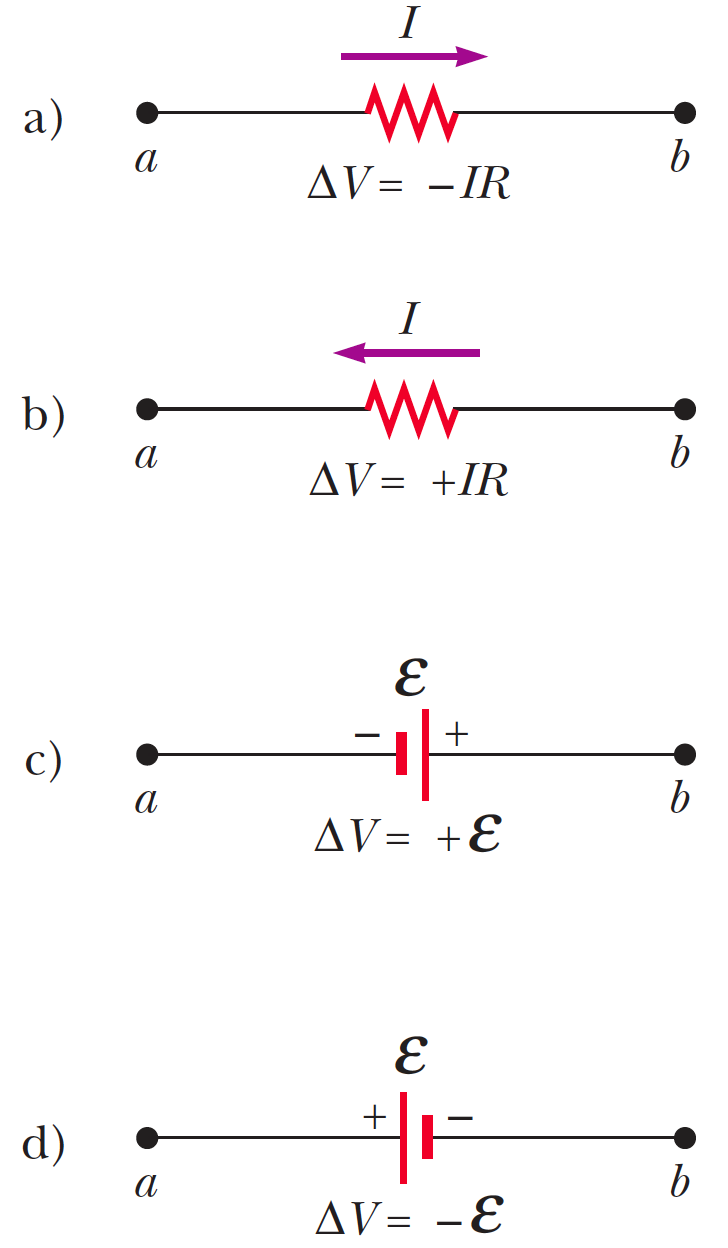
\includegraphics[width=0.4\textwidth]{4/figure_13}\par
      \end{multicols}

      \PN En general, para resolver un problema de circuito en particular, el número de ecuaciones independientes que se
      necesitan para obtener las dos leyes es igual al número de corrientes desconocidas.
